\documentclass[11pt,a4paper]{article}

% Enhanced packages for better typography and layout
\usepackage[left=0.75in, right=0.75in, top=0.75in, bottom=0.75in]{geometry}
\usepackage{hyperref}
\usepackage{enumitem}
\usepackage[usenames,dvipsnames]{xcolor}
\usepackage{fontspec}
\usepackage{setspace}
\usepackage[explicit]{titlesec}
\usepackage{multicol}
\usepackage{fontawesome5}
\usepackage{graphicx} % For including images

% Modern font selection
\setmainfont{Helvetica Neue}[
    UprightFont = *-Light,
    BoldFont = *-Bold,
]
\setsansfont{Arial}

% Custom colors
\definecolor{primarycolor}{RGB}{0, 79, 159}
\definecolor{secondarycolor}{RGB}{100, 100, 100}
\definecolor{linkcolor}{RGB}{0, 112, 201}
\definecolor{headerbg}{RGB}{240, 240, 240}

% Custom section styling
\titleformat{\section}
    {\LARGE\bfseries\color{primarycolor}\sffamily}
    {}{0em}
    {#1\hrule height 0.5pt \vspace{-1em}}

\titleformat{\subsection}
    {\bfseries\color{secondarycolor}\sffamily}
    {}{0em}{#1\vspace{-0.5em}}

% List styling
\setlist[itemize]{
    leftmargin=*,
    topsep=0.2em,
    itemsep=0.2em,
    parsep=0pt,
    label=\textbullet
}

% Hyperlink setup
\hypersetup{
    colorlinks=true,
    linkcolor=linkcolor,
    urlcolor=linkcolor,
    pdftitle={Evgeny Oleynik CV},
    pdfauthor={Evgeny Oleynik}
}

\begin{document}

% Header
\begin{center}
    \colorbox{headerbg}{\parbox{\textwidth}{
        \vspace{0.5em}
        \hspace{0.25em}
        \begin{minipage}[c]{0.2\textwidth}
            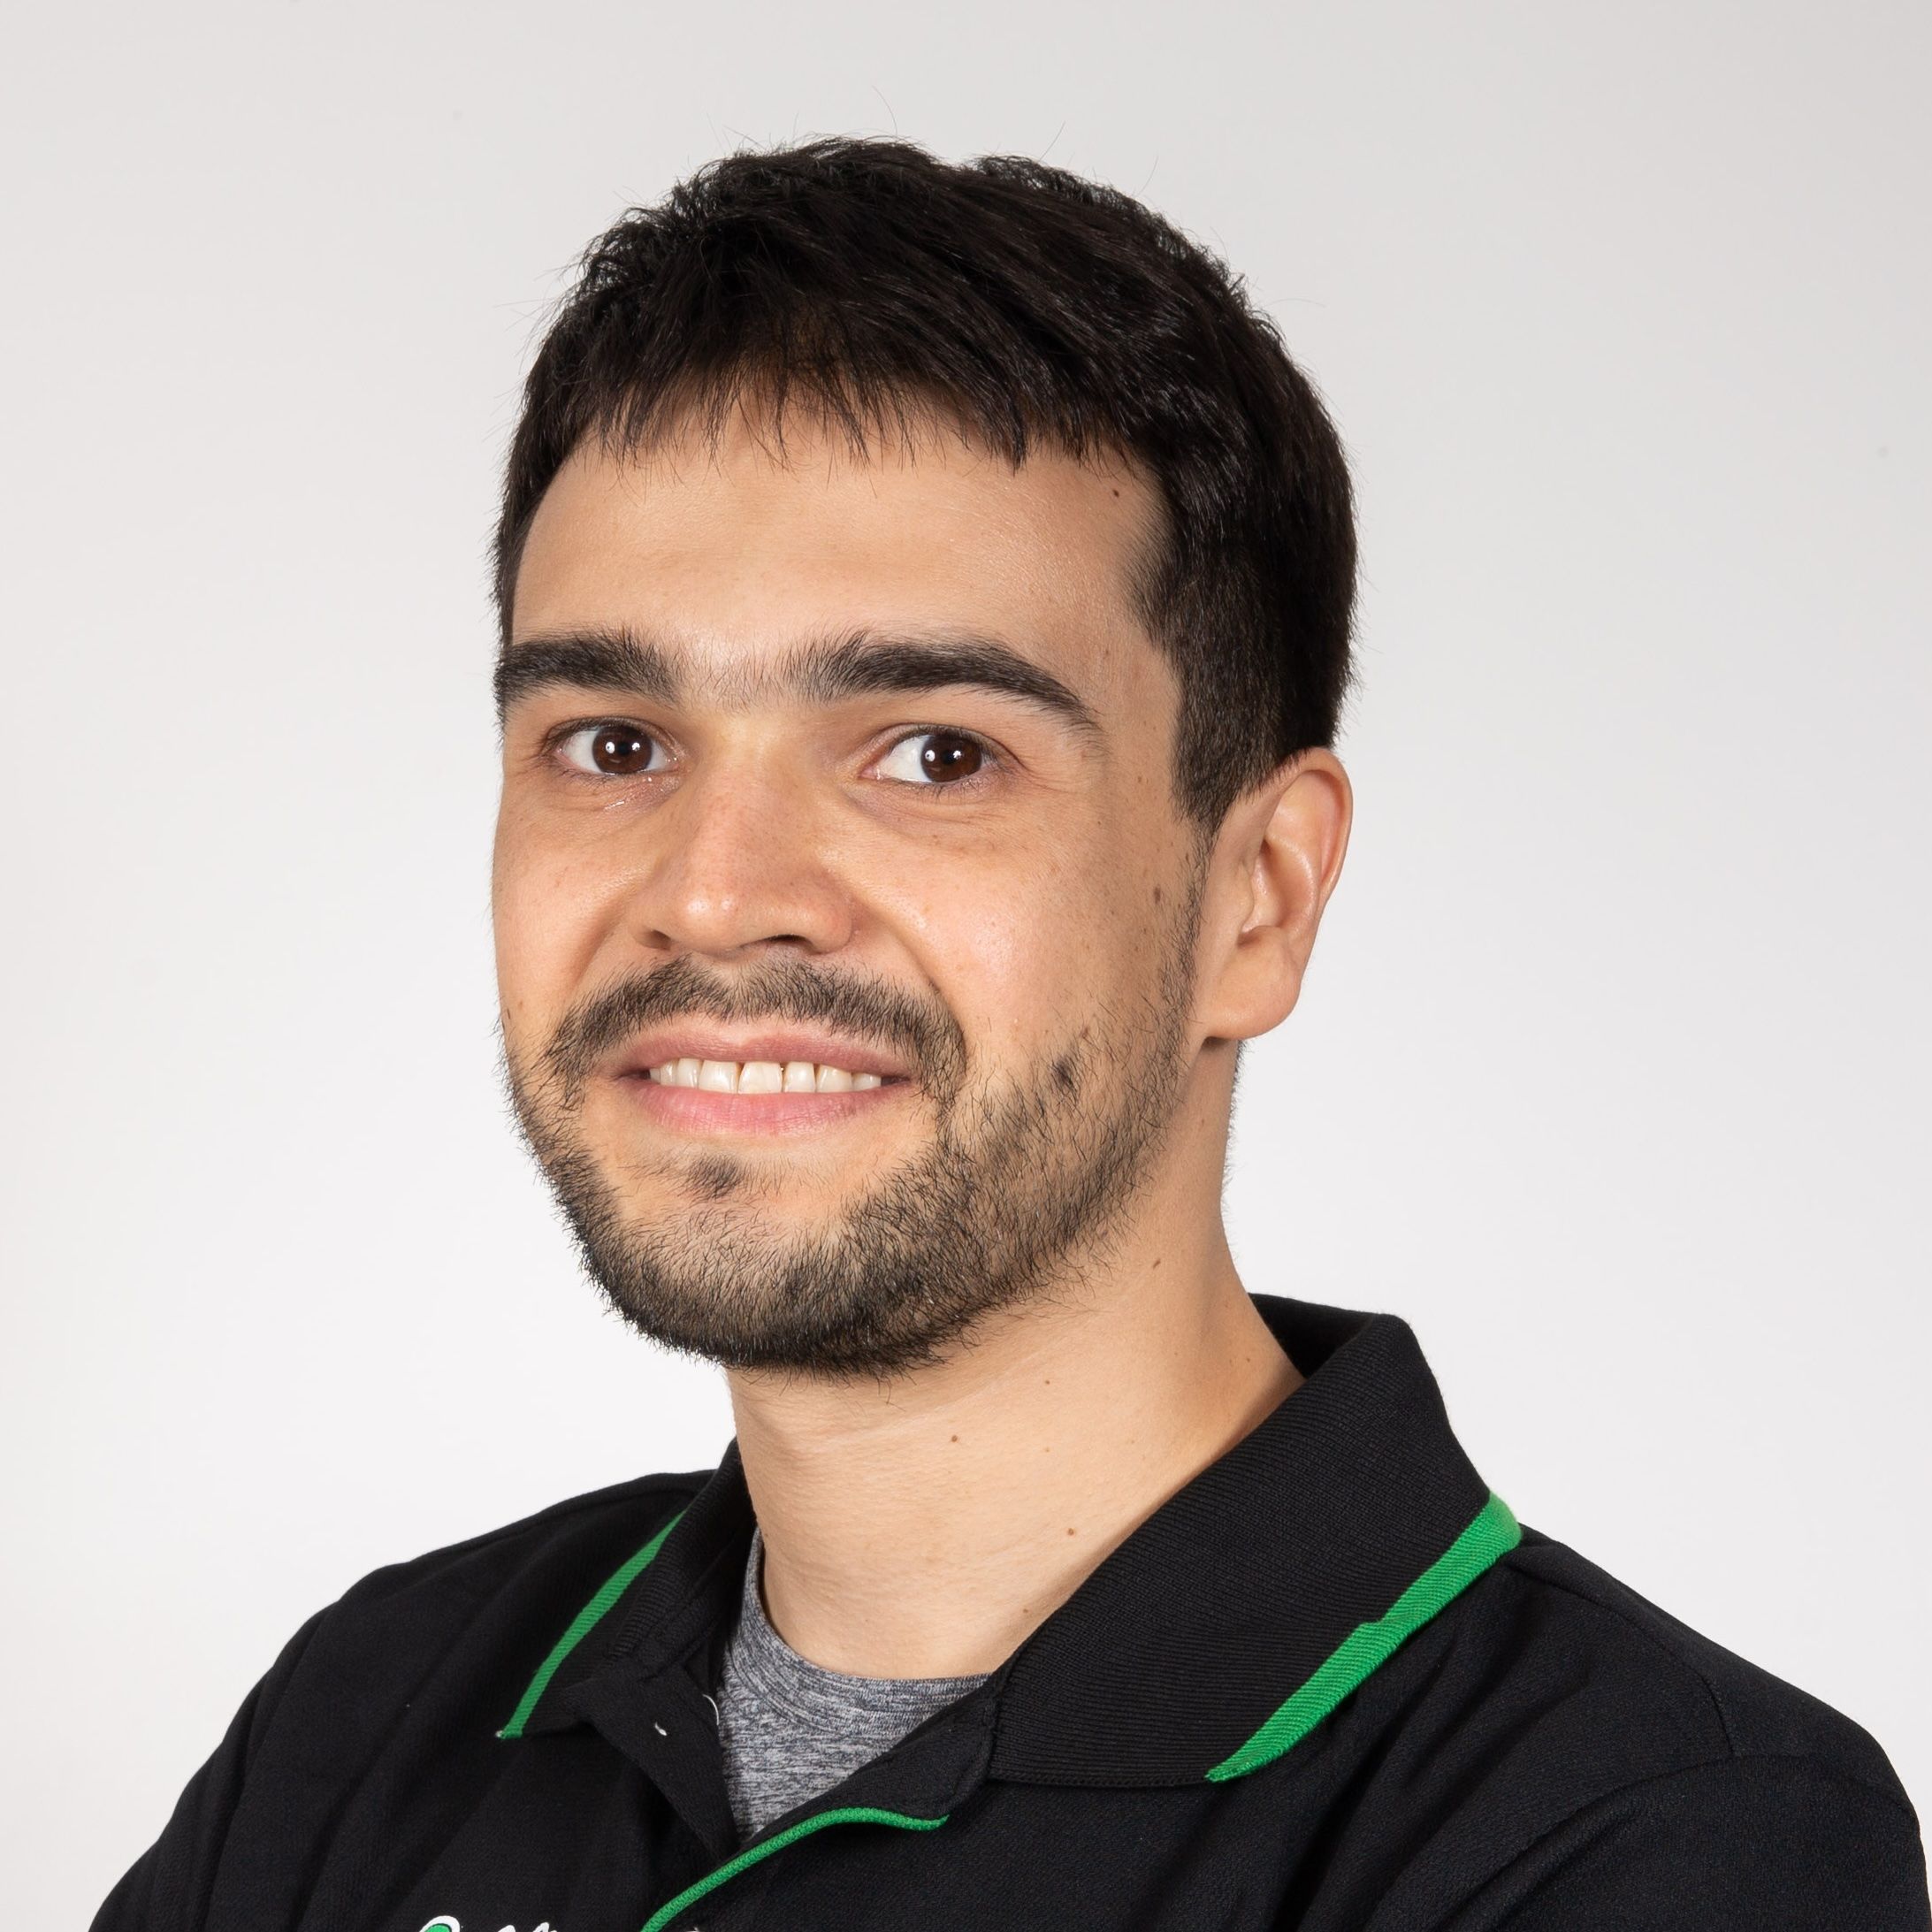
\includegraphics[width=\linewidth]{headshot.jpg} % Adjust the filename and path
        \end{minipage}\hspace{0.5em}\hfill
        \begin{minipage}[c]{0.75\textwidth}
            {\Huge\textbf{Evgeny Oleynik}} \\[0.3em]
            {\Large\color{secondarycolor} Co-Founder \& CTO, AirShelf AI | Permissionless Agentic Commerce} \\[0.5em]
            {\color{secondarycolor}
            \faMapMarker \, Singapore \\[0.2em]
            \faEnvelope \, \href{mailto:evoleinik@gmail.com}{evoleinik@gmail.com} | \faPhone \, +65 8272 3349 \\[0.2em]
            \faLinkedin \, \href{https://linkedin.com/in/evoleinik}{linkedin.com/in/evoleinik} | \faGithub \, \href{https://github.com/evoleinik}{github.com/evoleinik} | \faGlobe \, \href{https://airshelf.ai}{airshelf.ai}}
        \end{minipage}
        \vspace{0.5em}
    }}
\end{center}

% Professional Summary
\section*{Professional Summary}
{\setstretch{1.2}
Technical founder operating at the intersection of AI and commerce. Co-Founder \& CTO of AirShelf AI (Antler-backed, Singapore), making brands discoverable and transactable across AI assistants without platform gatekeepers. Previously Co-Founder \& CTO of 12Go --- APAC's leading ground transportation OTA, scaled to \textbf{50,000 bookings daily}, \textbf{45-person team}, and \textbf{\$500K daily GMV} over a decade.}

% Notable Achievements
\section*{Notable Achievements}
\begin{itemize}
    \item \textbf{Founded AirShelf AI} --- Antler-backed, selected for \textbf{HP Garage 2.0} APAC distribution. \textbf{13 merchants onboarded} in 7 months, including enterprise pilot with on-prem zero-data-leak inference.
    \item \textbf{Scaled 12Go} from startup to APAC's leading ground transportation OTA: \textbf{45-person remote team} across 12 departments, \textbf{\$500K daily GMV}, \textbf{99.95\% uptime}.
    \item \textbf{Navigated COVID-19} via operational pivots; led due diligence and post-merger integration for M\&A across \textbf{4 international markets}.
\end{itemize}

% Professional Experience
\section*{Professional Experience}

\subsection*{Co-Founder \& CTO \hfill Sep 2025--Present}
\textbf{AirShelf AI | Permissionless Agentic Commerce (Singapore)} \quad {\small\color{secondarycolor}\textit{Founded during Antler SG19; pre-seed funded}}
\begin{itemize}
    \item Built and shipped the full stack: edge infrastructure serving canonical AI surfaces, agent commerce protocol integration (ACP/UCP/MCP), and AI-discoverability primitives --- making any brand transactable across AI assistants without platform gatekeepers.
    \item Engineered \textbf{on-prem zero-data-leak inference} for enterprise customers, with fail-closed architecture so customer data never touches frontier APIs --- key differentiator for B2B compliance.
    \item Designed and shipped: merchant dashboard, semantic shopping API (\textbf{175+ stores / 22 markets}), AI-search visibility benchmarking across major assistants, hallucination detection, golden-record extraction pipeline.
    \item \textbf{13 merchants onboarded} in 7 months; selected for \textbf{HP Garage 2.0} APAC distribution.
\end{itemize}

\subsection*{Co-Founder \& Chief Technical Officer \hfill 2014--2025}
\textbf{12Go.com | Ground Transportation OTA (Online Travel)}
\begin{itemize}
    \item Scaled platform to \textbf{50,000 tickets sold daily}, \textbf{100+ searches/sec}, \textbf{<150ms search latency}, \textbf{99.95\% uptime}, global coverage.
    \item Built and led a \textbf{45-person remote team} across 12 departments spanning Eastern Europe, Southeast Asia, and the Middle East --- agile workflows, CI/CD, ICE-prioritized roadmap, A/B-tested product decisions.
    \item Architected the stack end-to-end: search API + sharded caches + pricing engine over \textbf{150+ supplier integrations}, web app (Vue.js, Nuxt) and a mobile app delivering \textbf{30\% of bookings} in year one, all on AWS (EC2, RDS, S3, CloudFront) with Grafana/Datadog/Clickhouse observability.
    \item Navigated COVID-19 via operational pivots; led due diligence and post-merger integration for the M\&A with an Israeli group, unifying operations across \textbf{Israel, Croatia, Argentina, and Brazil}.
\end{itemize}

\subsection*{Co-Founder \& CTO \hfill 2011--2012}
\textbf{GV | Holiday Rentals Platform (Online Travel)} --- Co-founded one of Southeast Asia's first holiday rental platforms; partnered with Airbnb during their Thailand expansion. Stack: PHP, MySQL, Go.

% Skills
\section*{Skills \& Expertise}
\begin{itemize}
    \item \textbf{AI \& LLM Integration}: Production systems across all major LLM providers (Anthropic, OpenAI, Google, Perplexity). On-prem GPU inference with open-source models. Semantic search, structured extraction, hallucination detection, agent commerce protocols (ACP, UCP, MCP).
    \item \textbf{Full-Stack}: TypeScript, Next.js, React, Node.js, PostgreSQL, Prisma, Redis, Vercel.
    \item \textbf{System Architecture}: Designing low-latency, high-availability systems. Edge proxies, API design, caching, real-time pipelines.
    \item \textbf{Cloud \& Infrastructure}: AWS (EC2, RDS, S3, CloudFront), Vercel, Neon (serverless Postgres), Docker, K3s. Monitoring: Grafana, Datadog, Axiom.
    \item \textbf{Leadership}: Built and managed 45-person remote team across 12 departments. Hiring, mentoring, retention. Agile, CI/CD, data-driven prioritization.
    \item \textbf{Founder Skills}: Fundraising (Antler pre-seed), enterprise sales, pilot delivery, investor relations, M\&A due diligence.
\end{itemize}

% Education
\section*{Education}
\textbf{Specialist degree in Applied Mathematics} (MSc-equivalent, 5-year programme) \\
Moscow Aviation Institute (National Research University) \hfill 2005--2010

% Additional Information
\section*{Additional Information}
\textbf{Languages:} Russian (native), English (fluent), Thai (conversational) \\
\textbf{Location:} Singapore (previously Bangkok, 10+ years)

\end{document}
